\section{Method}

% We divide AutoQ‑VIS into three key stages: (1) \textbf{Initial training} (\cref{sec:initial_model}), where we jointly pretrain a VideoMask2Former VIS model and a Mask‑Scoring‑R‑CNN–style quality predictor on synthetic videos from VideoCutLER; (2) \textbf{Multi‑round self‑training} (\cref{sec:multi_round_training}), in which we alternate between: (i) using the VIS model to generate pseudo‑labels on unlabeled videos, (ii) scoring each pseudo‑label by regressing its IoU via the quality predictor, and (iii)
% adding only those pseudo-labels back into the training set that are both confident and have high predicted IoU, as determined by a combined quality score exceeding a fixed threshold;
% and (3) \textbf{DropLoss for the mask head} (\cref{sec:droploss}), which dynamically suppresses loss contributions from any predicted mask whose maximum ground‑truth overlap falls below a small IoU threshold and enhances the mask head training.  Through this iterative, quality‑guided dataset augmentation, our pipeline progressively refines instance segmentation accuracy without requiring any human annotations.

AutoQ-VIS operates through four parts: (1) \textbf{Initial Training} (\cref{sec:initial_model}): Jointly pretrain VideoMask2Former and the mask quality predictor on VideoCutLER's synthetic videos; (2) \textbf{Multi-Round Self-Training} (\cref{sec:multi_round_training}): Iteratively generate pseudo-labels on real unlabeled videos, filter via quality scores, and augment training data; (3) \textbf{DropLoss} (\cref{sec:droploss}): Suppress low-IoU mask predictions to enhance mask head training. This quality-guided pipeline progressively improves segmentation accuracy without any human annotations; (4) \textbf{Adaptive fusion}: Augment the dataset dynamically through adaptive fusion of newly curated annotations.


% \dimpp{we need an initial paragraph here as an overview that explains the pipeline!}


\begin{figure}[t]
    \centering
    %\includegraphics[width=1\linewidth]{figures/quality_predictor.pdf}
    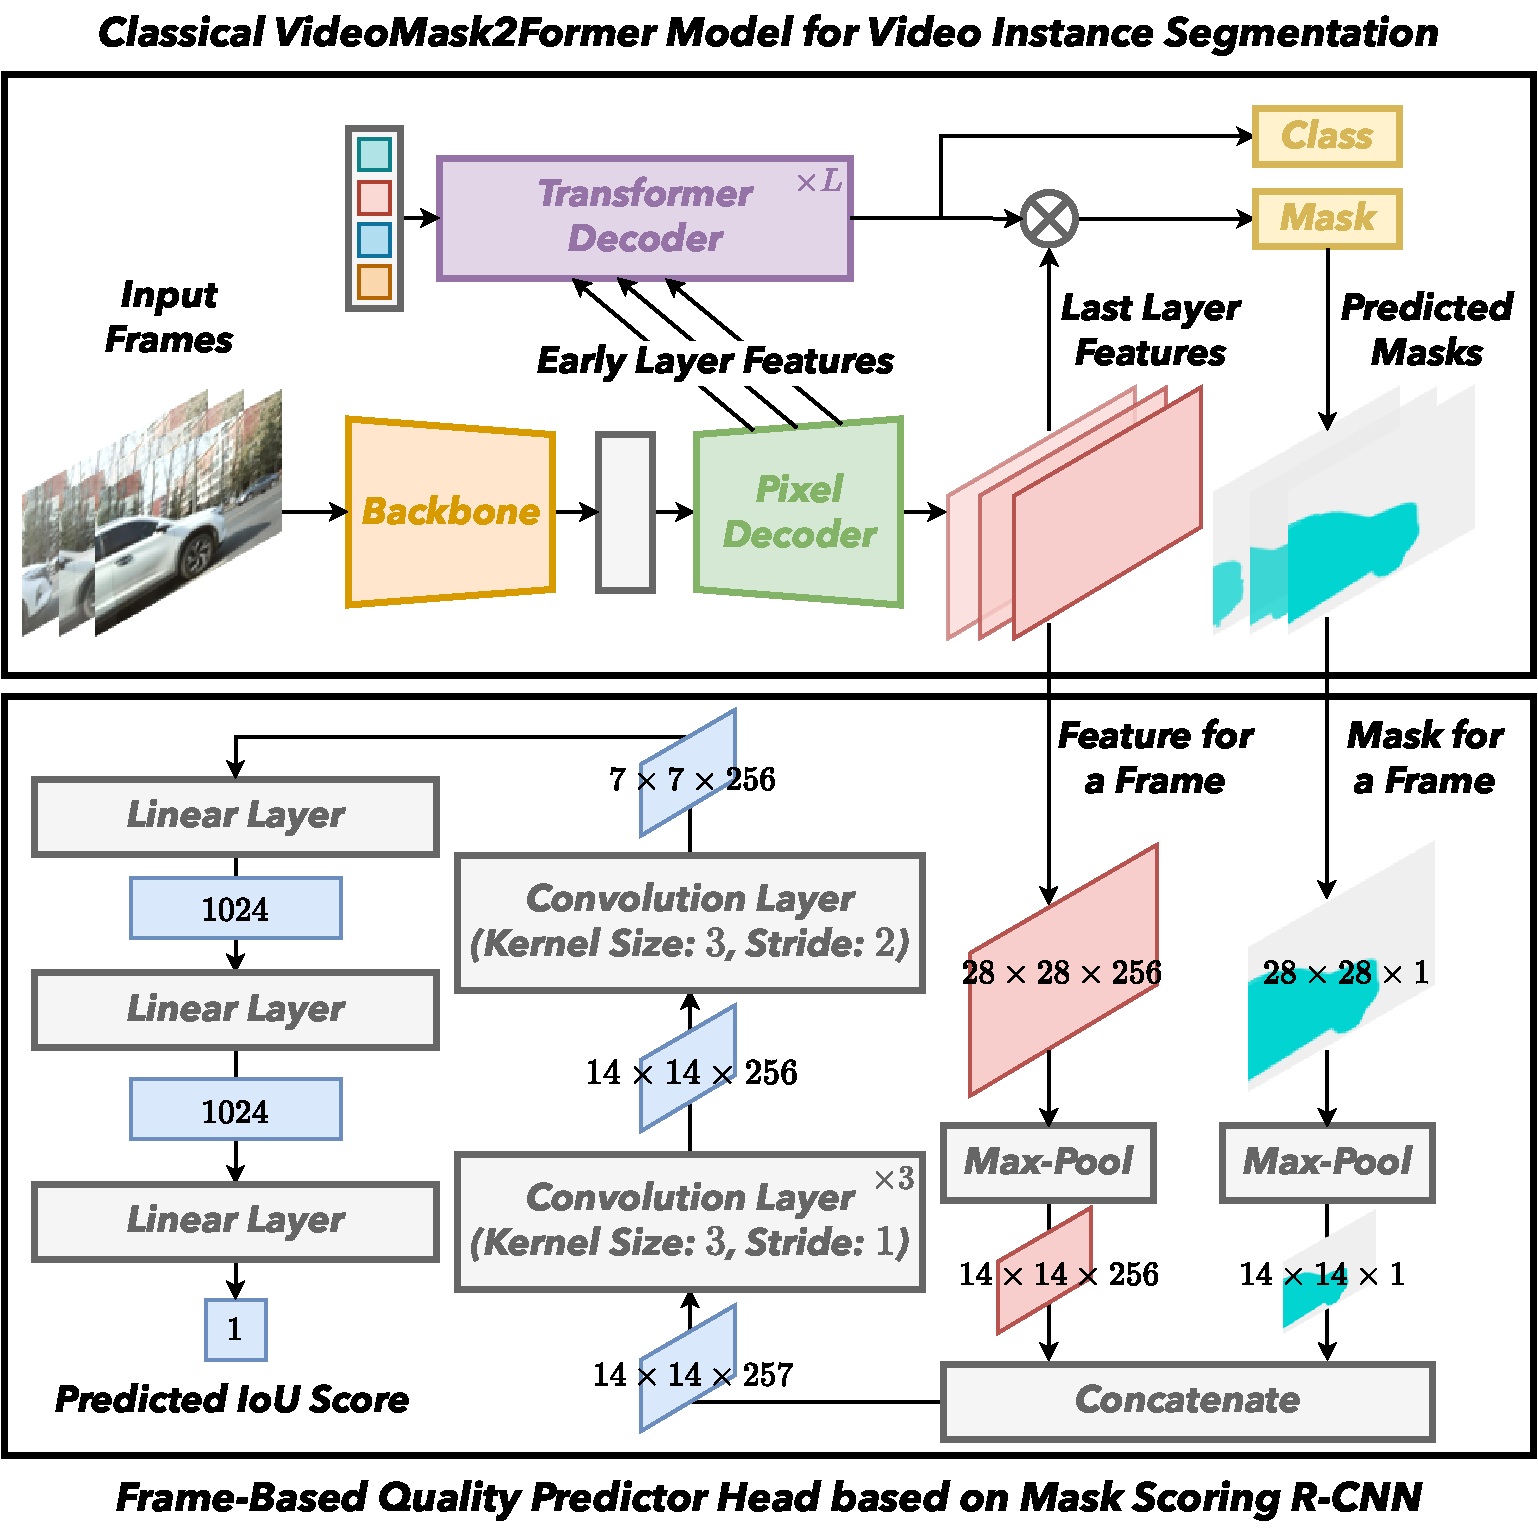
\includegraphics[width=1\linewidth]{figures/kaixuan_iccv_detailedarchitecture.pdf}
    \caption{
    \textbf{Network architecture of VideoMask2Former~\cite{mask2former, videomask2former} and Mask Quality Predictor.} Our quality predictor integrates mask predictions and pixel decoder features following~\cite{maskscore}, employing a sequential architecture with four convolution layers (3$\times$3 kernels, final layer stride of 2 for spatial reduction) followed by three fully-connected layers that ultimately produce mask IoU predictions.}
    \label{fig:predictor}
\end{figure}

% ONUR: I did not like this title. Call it "Initialization stage"?
%\subsection{Initialize VIS model and quality predictor}
%\subsection{Initialization stage}
\subsection{Initial training stage}
\label{sec:initial_model}

% \paragraph{Video instance segmentation (VIS) model.}
\mypar{Video instance segmentation (VIS) model.}
Following VideoCutLER~\cite{videocutler}, we use the VideoMask2Former~\cite{mask2former, videomask2former} with the ResNet-50~\cite{resnet} backbone as our video instance segmentation (VIS) model.

% \paragraph{Quality predictor.}
\mypar{Quality predictor.}
For the quality predictor, as shown in~\cref{fig:predictor}, we use an architecture
%very
inspired by Mask Scoring R-CNN~\cite{maskscore}. Our architecture processes individual frame features and single-object mask predictions per inference step. Supervision is established through threshold-binarized (0.5) mask IoU between predictions and matched ground truths, optimized via $\ell_2$ regression loss.
\kaixuan{I add the following sentences to highlight the difference between our quality predictor and the mask scoring}
Although the architecture of our quality predictor and Mask Scoring R-CNN is similar, there is a key difference between our model and theirs. In Mask Scoring R-CNN, the input predicted mask is threshold-binarized (0.5). In our case, we find it crucial to use the raw predicted mask instead of the threshold-binarized predicted mask. If we use the threshold-binarized predicted mask, the quality predictor cannot produce any meaningful output. 

% \paragraph{Synthetic videos.} 
\mypar{Synthetic videos.} 
VideoCutLER~\cite{videocutler} provides a high-quality pseudo-labeled synthetic video dataset that was built on the unlabeled images from ImageNet~\cite{imagenet}, which is very suitable to train and initialize our VIS model and quality predictor. We also use the trained VideoMask2Former model~\cite{videomask2former} from VideoCutLER to initialize our VIS model.
% Instead of freezing the VIS model and training the quality predictor only, we found that training them both can lead to higher IoU prediction accuracy. 

\subsection{Multi-round self-training}
\label{sec:multi_round_training}

As shown in \cref{fig:overall}, we optimize the VIS model through iterative self-training and dynamic dataset augmentation. The training dataset is initialized using the synthetic videos from VideoCutLER~\cite{videocutler}. Empirically, we find that executing model parameter restoration from the initial model weight (trained in \cref{sec:initial_model}) achieves a better performance.

After training the VIS model, we use the predicted masks on unlabeled videos with a confidence score over $0.25$ as pseudo-labels. Then we use the quality predictor to predict the IoU of each pseudo-label predicted mask. Let $\hat{\text{IoU}}_l$ denote the predicted IoU of label $l$, and $s_l$ denotes the confidence score of label $l$ from the class head of the VIS model (see~\cref{fig:predictor}). We define the quality score of label $l$ as $Q_l = \hat{\text{IoU}}_l \cdot s_l$.
% \begin{equation}
%     Q_l = \hat{\text{IoU}}_l \cdot s_l
% \end{equation}

We implement quality-based pseudo-label selection using a fixed quality score threshold $\tau_{\text{th}}$. For each pseudo-label $l$, we select it if $Q_l \geq \tau_{th}$. At the end of each round, we add all the pseudo-labels to the training dataset.

% ONUR: This may be a paragraph, instead of a subsection????

\subsection{DropLoss for mask head}
\label{sec:droploss}

We enhance the mask head training by suppressing loss contributions from low-overlap predictions, following CutLER~\cite{cutler}. For each predicted mask $m_i$, we discard its loss contribution if its maximum ground truth IoU falls below the threshold $\tau^{\text{IoU}}$:
\begin{equation}
    \mathcal{L}_{\text{drop}}(m_i) = \mathds{1}(\text{IoU}_i^{\text{max}} > \tau^{\text{IoU}})\mathcal{L}_{\text{vanilla}}(m_i)
\end{equation}

\noindent Here, $\text{IoU}_i^{\text{max}}$ is the maximum overlap between $m_i$ and any ground truth mask, while $\mathcal{L}_{\text{vanilla}}$ denotes the original mask head loss from VideoMask2Former~\cite{mask2former, videomask2former}. We employ a low threshold ($\tau^{\text{IoU}} = 0.01$) to filter only near-zero overlap predictions.

\subsection{Adaptive fusion of new curated annotations and old curated annotations}

To augment the training dataset, at the end of each round of self-training, we need to merge the old curated annotations in the training dataset with the new curated annotations.

The augmentation process operates in two distinct modes depending on whether the video containing the new detections already exists in the training set. For novel videos, we perform bulk insertion of all qualified detections. For existing videos, we implement an instance-level fusion protocol that intelligently merges new predictions with old annotations while preserving temporal consistency.

Let $d_v$ denote an object detection for video $v$, formally:
\begin{equation}
    d_v = \{(S^t, m^t)\}_t^{T_v} 
\end{equation}
Here, $S^t \in \{0, 1\}$ indicates whether the object mask (pseudo label) of $d_v$ at frame $t$ is selected for self-training, $m^t$ denotes the binary object mask at frame $t$.


Let $\mathcal{T}^{(k)} = \{(v, \mathcal{D}_v)\}$ denote the training dataset at iteration $k$, where $\mathcal{D}_v$ contains all preserved detections (old annotations) for video $v$, and $\mathcal{D}_{\text{retained}}^{(k)}$ denote the set of detections that we retained after the filtering using the quality score threshold $\tau_{th}$ at the end of iteration $k$ (new detections). We need to merge the $\mathcal{D}_{\text{retained}}^{(k)}$ into the $\mathcal{T}^{(k)} = \{(v, \mathcal{D}_v)\}$. For each video, if it's not in the training dataset, we simply add all its detections to the training dataset. Formally, let $\mathcal{D}_{\text{retained},v}^{(k)}$ denote the detections belong to video $v$:
\begin{equation}
    \mathcal{D}_{\text{retained},v}^{(k)} = \left\{ d \in \mathcal{D}_{\text{retained}}^{(k)} \,\big|\, d \text{ belongs to video } v \right\}
\end{equation}

Let $\mathcal{V}_{\text{new}}^{(k)} = \pi_1(\mathcal{D}_{\text{retained}}^{(k)}) \setminus \pi_1(\mathcal{T}^{(k)})$ denote completely new videos, where $\pi_1$ projects to video identifiers. Let $\mathcal{T}_{\text{new}}^{(k)}$ denote labels of new videos:

\begin{equation}
\mathcal{T}_{\text{new}}^{(k+1)} =  \bigcup_{v \in \mathcal{V}_{\text{new}}^{(k)}} \left\{ \left(v, \mathcal{D}_{\text{retained},v}^{(k)} \right) \right\}
\end{equation}

For videos already present in the training set, we implement a temporal-aware fusion protocol that resolves conflicts between new detections and old annotations.

To merge the existing detections and new detections, we need to identify whether two detections overlap. We define the spatiotemporal overlap predicate for two detections:
\begin{equation}
    \phi(d_{\text{new}, v}, d_{\text{exist}, v}) \triangleq \exists t \in [1, T_v]: \frac{\|m_{\text{new}}^t \cap m_{\text{exist}}^t\|}{\|m_{\text{new}}^t \cup m_{\text{exist}}^t\|} \geq 0.5
\end{equation}

% This predicate is very similar to what we use in spatiotemporal NMS.
If in any frames, two detections' masks overlap (IoU $\geq$ 0.5), we consider them overlapping detections. If two detections overlap, we need to fuse them. We fuse the new detection and the existing detection frame by frame. For one frame, if only the existing detection's label is selected, we use its label; otherwise, we use the new detection's label. Let $\mathcal{F}$ denote the fusion operation:
\begin{equation}
    \mathcal{F}(d_{\text{new},v}, d_{\text{exist},v}) =  \{\mathcal{S}_{\text{merge}}^t, m_{\text{merge}}^t\}_{t=1}^{T_v}
\end{equation}
where:
\begin{equation}
    \mathcal{S}_{\text{merge}}^t = \max(\mathcal{S}_{\text{new}}^t, \mathcal{S}_{\text{exist}}^t)
\end{equation}
\begin{equation}
    m_{\text{merge}}^t = \begin{cases} 
m_{\text{exist}}^t & \text{if } \mathcal{S}_{\text{exist}}^t = 1 \land \mathcal{S}_{\text{new}}^t = 0 \\
m_{\text{new}}^t & \text{otherwise}
\end{cases}
\end{equation}

If the new detection does not overlap with any existing detections, we simply add it. Let $\mathcal{V}_{\text{exist}}^{(k)} = \pi_1(\mathcal{T}^{(k)})$ denote existing videos. For each existing video $v \in \mathcal{V}_{\text{exist}}^{(k)}$, we process all new detections $\mathcal{D}_{\text{retained},v}^{(k)}$ through:
\begin{equation}
    \mathcal{D}_v^{(k+1)} = \mathcal{D}_v^{(k)} \bigoplus \mathcal{D}_{\text{retained},v}^{(k)}
\end{equation}
where the operation $\bigoplus$ is defined as:
\begin{equation}
    \mathcal{D} \bigoplus \mathcal{D}' = \bigcup_{d' \in \mathcal{D}'} \left( \mathcal{D} \oplus d' \right)
\end{equation}
with per-detection fusion:
\begin{equation}
\mathcal{D} \oplus d_{\text{new}} = 
\begin{cases}
\mathcal{D} \cup \{d_{\text{new}}\} & \text{if } \forall d_{\text{exist}} \in \mathcal{D}, \\
& \quad \neg\phi(d_{\text{new}}, d_{\text{exist}}) \\
\mathcal{D} \setminus d_{\text{exist}} \cup \mathcal{F}(d_{\text{new}}, d_{\text{exist}}) & \text{if } \exists d_{\text{exist}} \in \mathcal{D}, \\
& \quad \phi(d_{\text{new}}, d_{\text{exist}})
\end{cases}
\end{equation}

In the end, we merge the labels of new videos and existing videos:
\begin{equation}
    \mathcal{T}^{(k+1)} = \mathcal{T}_{\text{new}}^{(k+1)} \cup \mathcal{T}_{\text{exist}}^{(k+1)}
\end{equation}
where:
\begin{equation}
    \mathcal{T}_{\text{exist}}^{(k+1)} =  \bigcup_{v \in \mathcal{V}_{\text{exist}}^{(k)}} \left\{ \left(v, \mathcal{D}_{v}^{(k+1)} \right) \right\}
\end{equation}

During training, for each video, we need to sample three frames as the input of the model (following VideoCutLER~\cite{videocutler}). To provide good-quality labels, we only sample those frames where all their detections are selected. For each video $v \in \mathcal{V}_{\text{train}}^{(k+1)}$, we define the eligible frame set:
\begin{equation}
\mathcal{F}_{\text{eligible}}^{(k+1)}(v) = \left\{ t \in [1,T_v] \,\big|\, \forall d \in \mathcal{D}_v^{(k+1)}: \mathcal{S}_d^t = 1 \right\}
\end{equation}

The training batch is constructed through uniform sampling:
\begin{equation}
\mathcal{B}_{\text{train}}^{(k+1)}(v) = \mathop{\mathrm{UniformSample}}\limits_{3} \left( \mathcal{F}_{\text{eligible}}^{(k+1)}(v) \right)
\end{equation}

Although we only use a subset of pseudo-labels, all pseudo-labels persist in the training set regardless of selection status, enabling progressive refinement.

% To balance data distribution between VideoCutLER's~\cite{videocutler} extensive synthetic videos and our pseudo-labeled videos, we implement a balanced stochastic sampling strategy. Each training batch has an equal probability (50\%) of being drawn from either the synthetic videos or the pseudo-labeled set. This prevents overfitting to either domain while maintaining the synthetic data's regularization benefits during self-training. \todo{move it to implement detail}



% ONUR: No need for the YoutubeVIS row, always the same eval set
\begin{table}[!t]
\resizebox{\columnwidth}{!}{%
\begin{tabular}{lrrrrrrr}
\toprule

\multicolumn{1}{c}{}                                 & \multicolumn{7}{c}{\textbf{YouTubeVIS-2019}}   \\  \cline{2-8}
\multicolumn{1}{c}{\multirow{-2}{*}{\textbf{Method}}} &
  \multicolumn{1}{l}{\textbf{${\text{AP}}_{50}$}} &
  \multicolumn{1}{l}{\textbf{${\text{AP}}_{75}$}} &
  \multicolumn{1}{l}{\textbf{${\text{AP}}$}} &
  \multicolumn{1}{l}{\textbf{${\text{AP}}_{S}$}} &
  \multicolumn{1}{l}{\textbf{${\text{AP}}_{M}$}} &
  \multicolumn{1}{l}{\textbf{${\text{AP}}_{L}$}} &
  \multicolumn{1}{l}{\textbf{${\text{AR}}_{10}$}} \\ \midrule

% \textbf{Method} & 
% \textbf{${\text{AP}}_{50}$} &
% \textbf{${\text{AP}}_{75}$} &
% \textbf{${\text{AP}}$} & 
% \textbf{${\text{AP}}_{S}$} & 
% \textbf{${\text{AP}}_{M}$} & 
% \textbf{${\text{AP}}_{L}$} & 
% \textbf{${\text{AR}}_{10}$} \\ \midrule

MotionGroup~\cite{motiongroup} & 0.5  & 0.0  & 0.1  & 0.0 & 0.4  & 0.1  & 1.2  \\
OCLR~\cite{oclr}               & 5.5  & 0.3  & 1.6  & 0.1 & 1.6  & 6.1  & 11.5 \\
CutLER~\cite{cutler}           & 36.4 & 13.5 & 16.0 & 3.5 & 13.9 & 26.0 & 29.8 \\
VideoCutLER~\cite{videocutler} & 48.2 & 22.9 & 24.5 & 6.7 & 17.7 & 36.3 & 42.3 \\
AutoQ-VIS                                           & 52.6 & 28.2 & 28.1 & 6.7 & 21.2 & 40.7 & 42.5 \\
\textit{vs. previous SOTA} &
  {\color[HTML]{009901} +4.4} &
  {\color[HTML]{009901} +5.3} &
  {\color[HTML]{009901} +3.6} &
  {\color[HTML]{009901} +0.0} &
  {\color[HTML]{009901} +3.5} &
  {\color[HTML]{009901} +4.4} &
  {\color[HTML]{009901} +0.2} \\

\bottomrule
\end{tabular}%
}
\caption{
\textbf{YouTubeVIS-2019 \texttt{val}.} We reproduced MotionGroup~\cite{motiongroup}, OCLR~\cite{oclr}, CutLER~\cite{cutler}, and VideoCutLER~\cite{videocutler} results with the official code and checkpoints. AutoQ-VIS outperforms the state-of-the-art VideoCutLER by 4.4 $\text{AP}_{50}$. We evaluate results on YouTubeVIS-2019's \texttt{val} split in a class-agnostic manner.
}
\label{tab:ytvis19val}
\end{table}